\documentclass[conference]{IEEEtran}
\IEEEoverridecommandlockouts
% The preceding line is only needed to identify funding in the first footnote. If that is unneeded, please comment it out.
\usepackage{cite}
\usepackage{amsmath,amssymb,amsfonts}
\usepackage{algorithmic}
\usepackage{graphicx}
\usepackage{textcomp}
\usepackage{xcolor}
\usepackage{ctex}
\usepackage{fontspec}
\usepackage{listings}

\def\BibTeX{{\rm B\kern-.05em{\sc i\kern-.025em b}\kern-.08em
    T\kern-.1667em\lower.7ex\hbox{E}\kern-.125emX}}
\begin{document}

\title{数字图像处理实践报告}

\author{\IEEEauthorblockN{黄润华}
\IEEEauthorblockA{\textit{中国海洋大学} \\
huangrunhua@stu.ouc.edu.cn}}

\maketitle

\begin{abstract}
本报告为数字图像处理课程中期实践报告,内容涵盖图像增强、图像去噪、边窗滤波与维纳滤波等。报告内仿真内容部分均采用Matlab编程语言实现,仿真软件环境为Matlab R2021b,设备处理器为Apple M1,运行内存为16GB。
\end{abstract}

\begin{IEEEkeywords}
    image enhancement, image denoising, side window filter, Wiener filter
\end{IEEEkeywords}

\section{实践内容}
\begin{itemize}
    \item[1.] 任意选择一个灰度图像,应用全局直方图均衡化进行图像增强;用自适应直方图均衡化方法 (AHE)进行图像增强,改变局部图像块的大小,讨论结果的不同。
    \item[2.]选择测试图像(Iena 灰度图或其它),添加高斯噪声(低,中高水平),运用下列几种方式去噪:高斯低通, 小波去噪, 双边滤波,非局部均值.
    \item[3.] 查找有关“边窗滤波”的文献和算法实现,要求:简要叙述其原理;进行实验验证(任意选择测试图像,与任务2的结果比较) 
    \item[4.] 选择测试图像(Lena 灰度图或其它),经高斯低通滤波变模糊,再加上高斯噪声后成为退化图像,应用维纳滤波复原方法对其复原,给出不同噪声水平下的复原结果 
\end{itemize}

\section{仿真结果}
\subsection{全局直方图均衡化结果}
\begin{figure}[htbp]
	\centerline{
		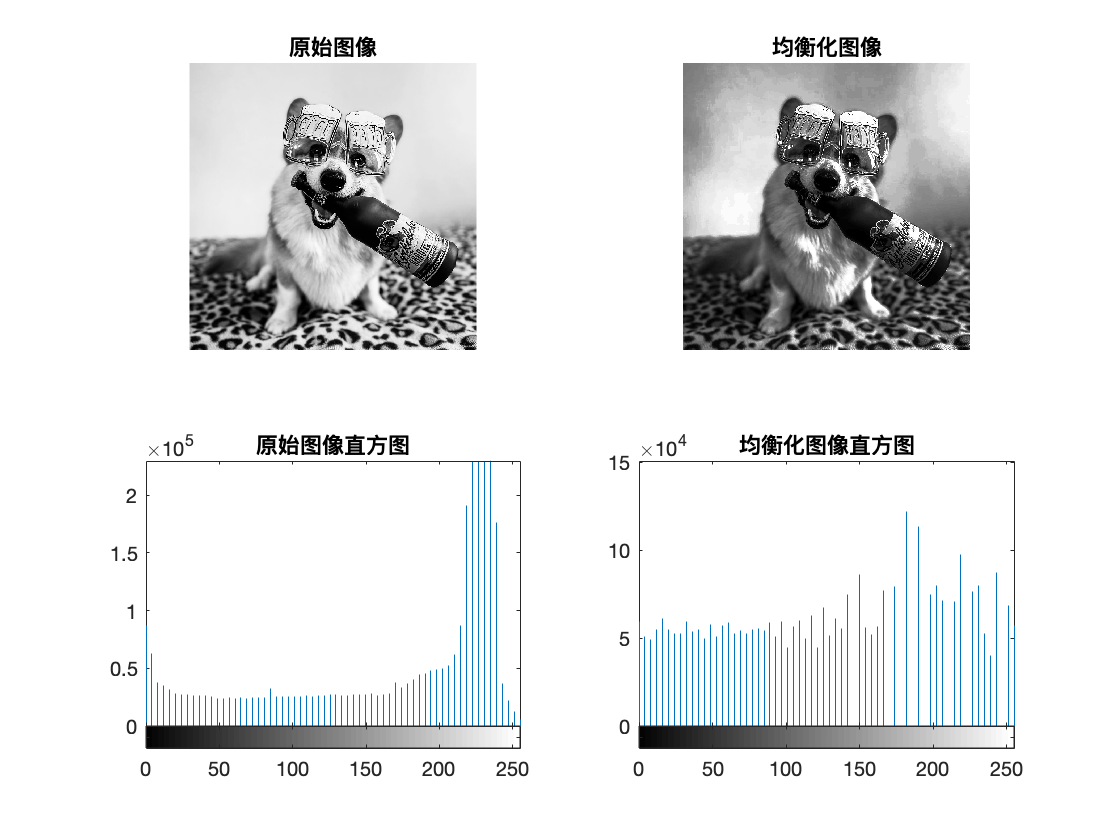
\includegraphics[width=9cm]{q1_1.png} 	
	}
	\caption{全局直方图均衡化结果}
	\label{pic1}
\end{figure}

图\ref{pic1}显示了应用全局直方图均衡化\cite{b1}进行图像增强的最终结果。其中第一行图片分别代表原始灰度图像与直方图均衡化后的图像;第二行分别显示了直方图均衡化前后图像的直方图信息。从直方图可以直观的看出在进行直方图均衡化后,原始图像的直方图变成均匀分布的形式,同时从图像本身对比可以发现,添加直方图均衡化后的图像整体对比度效果明显增强。

\subsection{自适应直方图均衡化结果}
\begin{figure}[htbp]
	\centerline{
		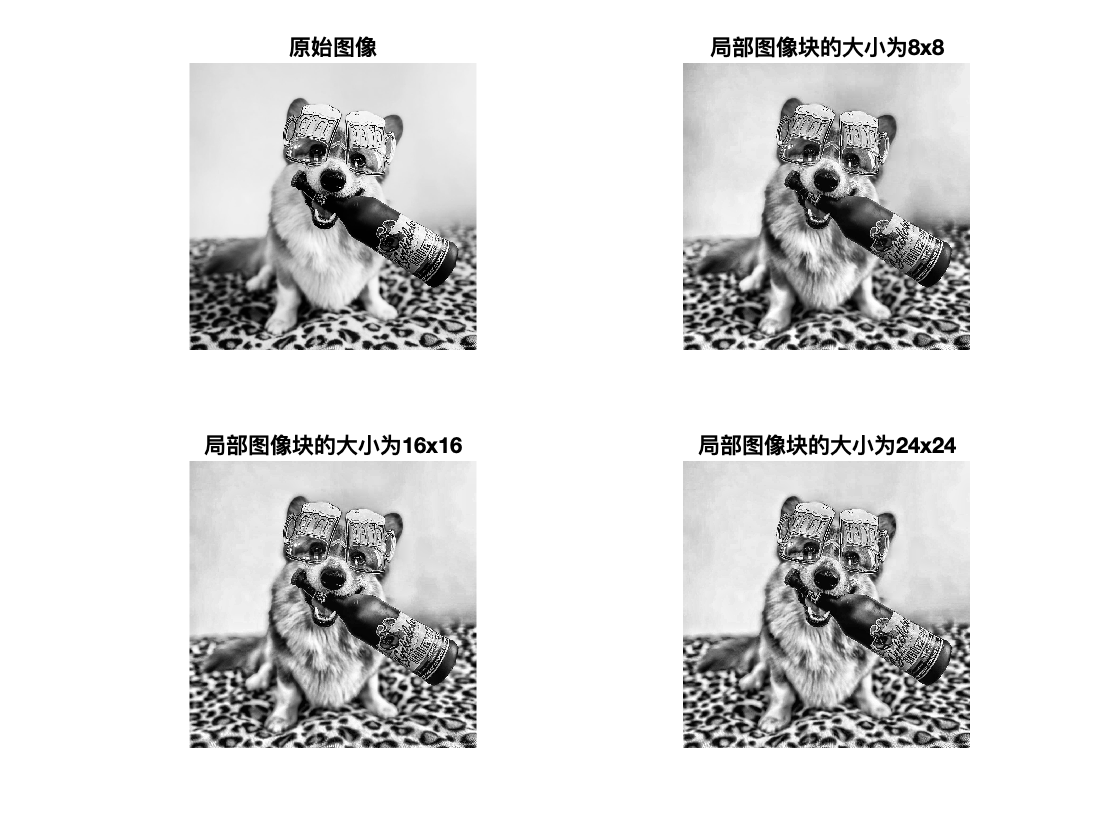
\includegraphics[width=9cm]{q1_2.png} 	
	}
	\caption{自适应直方图均衡化结果}
	\label{pic2}
\end{figure}

图\ref{pic2}显示了应用自适应直方图均衡化\cite{b2}进行图像增强的最终结果。其中第一行图片分别代表原始灰度图像与采用局部图像块大小为$8\times 8$自适应直方图均衡化后的图像;第二行分别为采用局部图像块大小为$16\times 16$自适应直方图均衡化后的图像与采用局部图像块大小为$24\times 24$自适应直方图均衡化后的图像。

通过图像的对比可以看出使用自适应直方图均衡化方法后图像的局部对比度增强,同时图像细节更加细腻饱满。同时,随着采用的局部图像块大小的增大,图像的细节随之增多,局部对比度也呈现正相关的增长。这表明自适应直方图均衡化方法适合于改进图像的局部对比度以及获得更多的图像细节。

\subsection{高斯低通滤波去噪结果}
\begin{figure}[htbp]
	\centerline{
		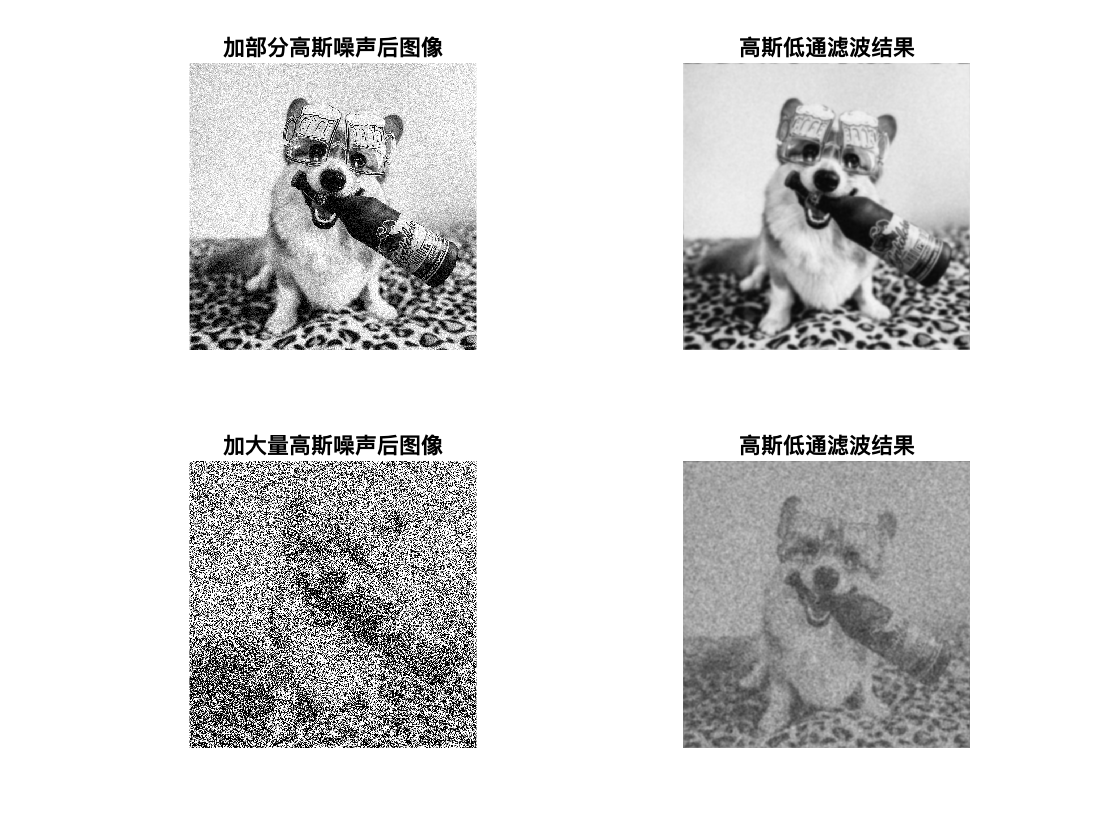
\includegraphics[width=9cm]{GL.png} 	
	}
	\caption{高斯低通滤波去噪结果}
	\label{pic3}
\end{figure}

图\ref{pic3}左边一列显示了对灰度图像添加不同水平的高斯噪声后的结果,可以明显看出,随着加入的高斯噪声的增多,图片的模糊程度逐渐增加,图片愈发难以辨认。

图\ref{pic3}右边一列显示了添加高斯噪声后的灰度图片进行高斯低通滤波的结果。通过对比第一行两张图片可以看出,经过高斯低通滤波后的图像去除了较多的噪点,保留了原始图片较多的细节,但出现了边际模糊的现象。在处理含有大量噪声的图片时,高斯低通对图像噪声的抑制较为明显,同时滤波后的图像具备原始图像的大致轮廓。

\subsection{小波去噪结果}
\begin{figure}[htbp]
	\centerline{
		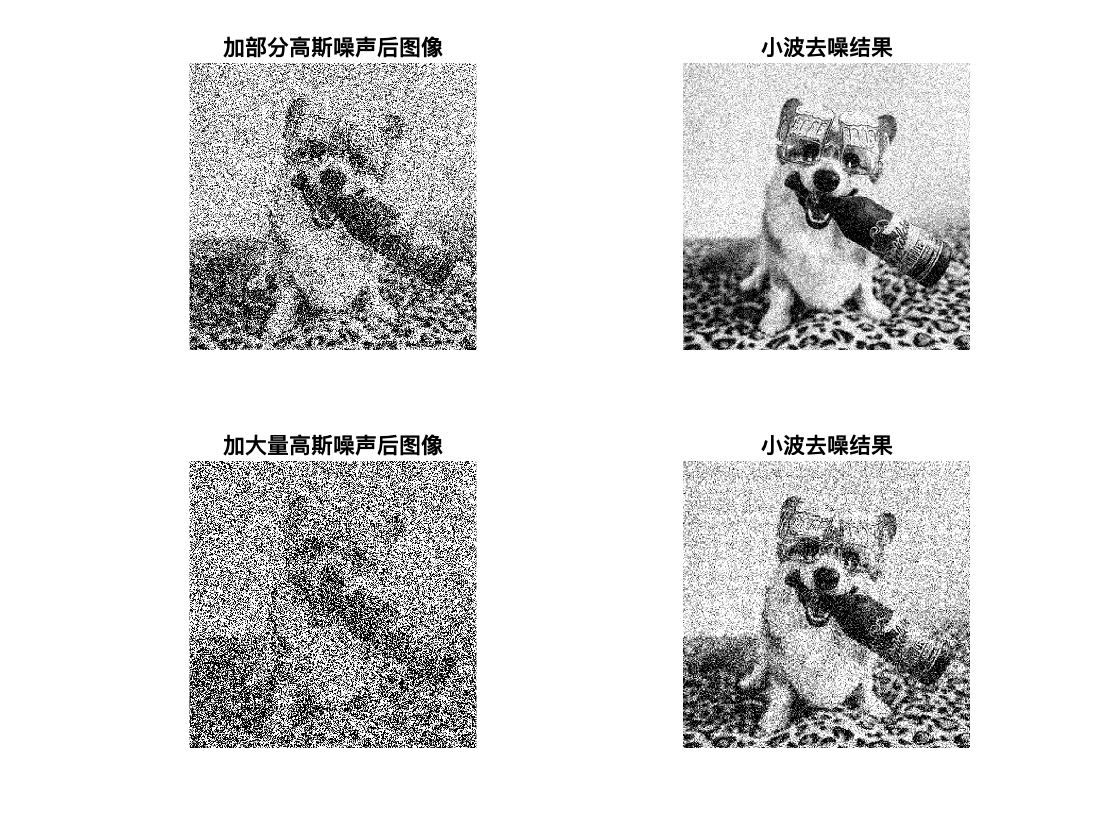
\includegraphics[width=9cm]{LW滤波结果.png} 	
	}
	\caption{小波去噪结果}
	\label{pic4}
\end{figure}

图\ref{pic4}左边一列显示了对灰度图像添加不同水平的高斯噪声后的结果,可以明显看出,随着加入的高斯噪声的增多,图片的模糊程度逐渐增加,图片愈发难以辨认。

图\ref{pic4}右边一列显示了添加高斯噪声后的灰度图片进行小波去噪\cite{b3}的结果。通过对比第一行两张图片可以看出,经过小波去噪后的图像去除了较多的噪点,保留了原始图片较多的细节。在处理含有大量噪声的图片时,小波去噪对图像噪声的抑制较为明显,同时滤波后的图像具备原始图像的大致轮廓。对比图\ref{pic4}与图\ref{pic3}的第二行可以发现,相比于高斯低通滤波的方法,小波去噪对图像噪声的抑制较为明显。

\subsection{双边滤波结果}
\begin{figure}[htbp]
	\centerline{
		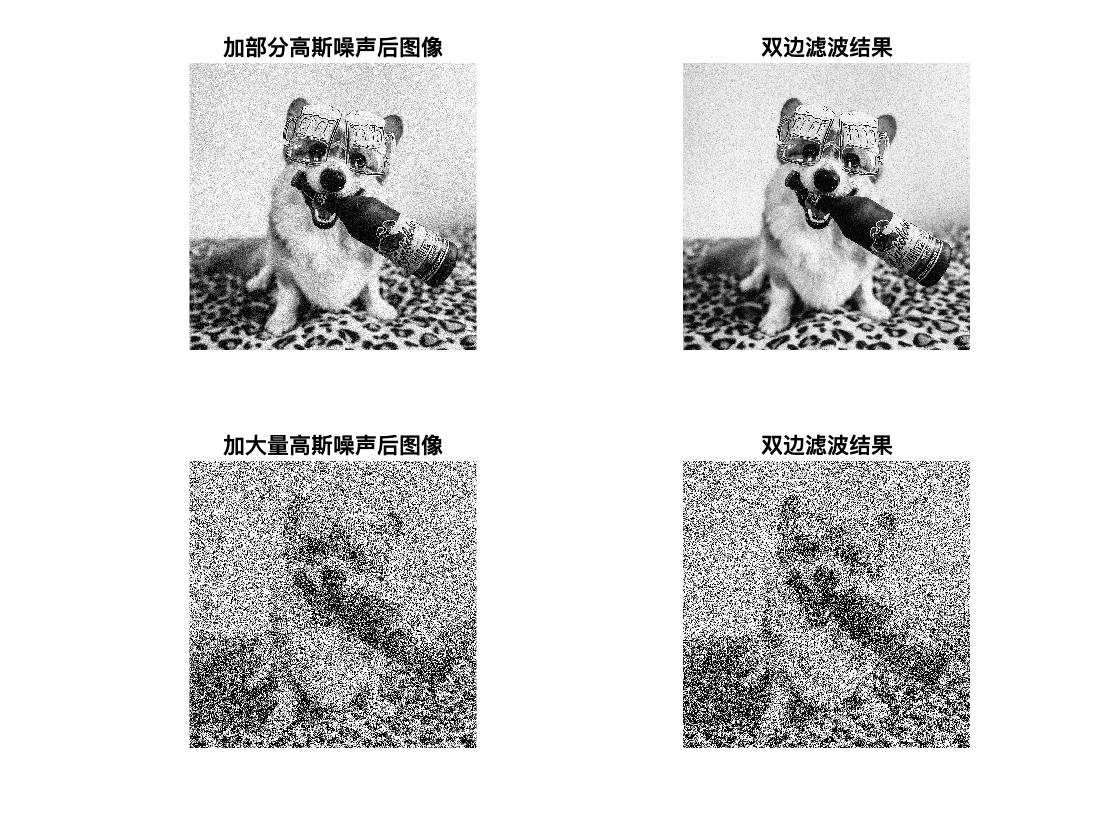
\includegraphics[width=9cm]{DF滤波结果.png} 	
	}
	\caption{双边滤波结果}
	\label{pic5}
\end{figure}

图\ref{pic5}左边一列显示了对灰度图像添加不同水平的高斯噪声后的结果,可以明显看出,随着加入的高斯噪声的增多,图片的模糊程度逐渐增加,图片愈发难以辨认。

图\ref{pic5}右边一列显示了添加高斯噪声后的灰度图片进行双边滤波\cite{b4}的结果。通过对比第一行两张图片可以看出,经过双边滤波后的图像去除了较多的噪点,保留了原始图片较多的细节。同高斯低通滤波相比,双边滤波后的图像没有出现图片边缘模糊化的现象。然而在处理含有大量噪声的图片时,双边滤波对图像噪声的抑制较差。

\subsection{非局部均值滤波结果}
\begin{figure}[htbp]
	\centerline{
		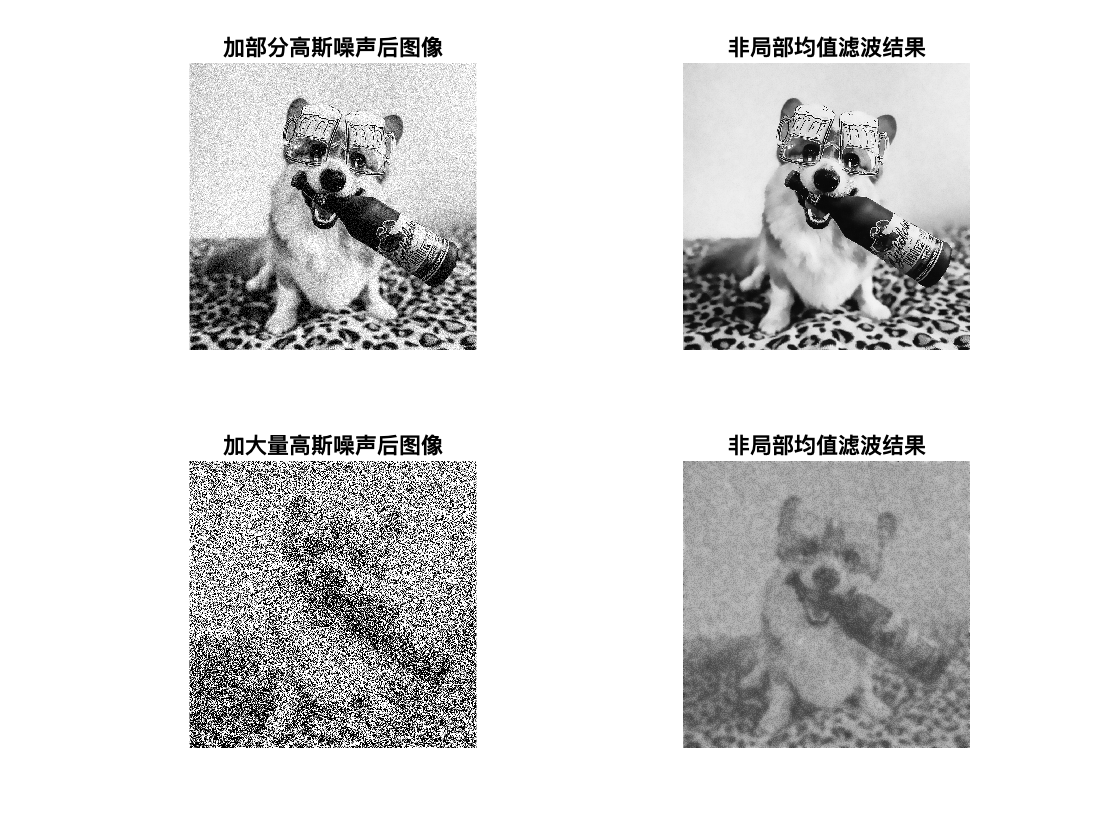
\includegraphics[width=9cm]{NLM滤波结果.png} 	
	}
	\caption{非局部均值滤波结果}
	\label{pic6}
\end{figure}

图\ref{pic6}左边一列显示了对灰度图像添加不同水平的高斯噪声后的结果,可以明显看出,随着加入的高斯噪声的增多,图片的模糊程度逐渐增加,图片愈发难以辨认。

图\ref{pic6}右边一列显示了添加高斯噪声后的灰度图片进行非局部均值滤波\cite{b5}的结果。通过对比第一行两张图片可以看出,经过非局部均值滤波后的图像去除了较多的噪点,保留了原始图片较多的细节。同高斯低通滤波相比,非局部均值滤波后的图像没有出现图片边缘模糊化的现象。在处理含有大量噪声的图片时,非局部均值滤波后的图像可以大致反映原始图像的轮廓。

\section{边窗滤波}
\subsection{边窗滤波原理}
边窗滤波\cite{b6}本质上为保边滤波策略,核心思想在于将每个滤波像素点都当成是潜在的边缘点,对于每个待滤波的像素点,生成几种不同的滤波子窗口,将生成的滤波子窗口的边缘或者角点位置同待滤波的像素点对齐,进行滤波得到结果,根据子窗口的滤波之后的最佳重构结果作为最终的滤波结果。

\subsection{边窗滤波仿真结果}
\begin{figure}[htbp]
	\centerline{
		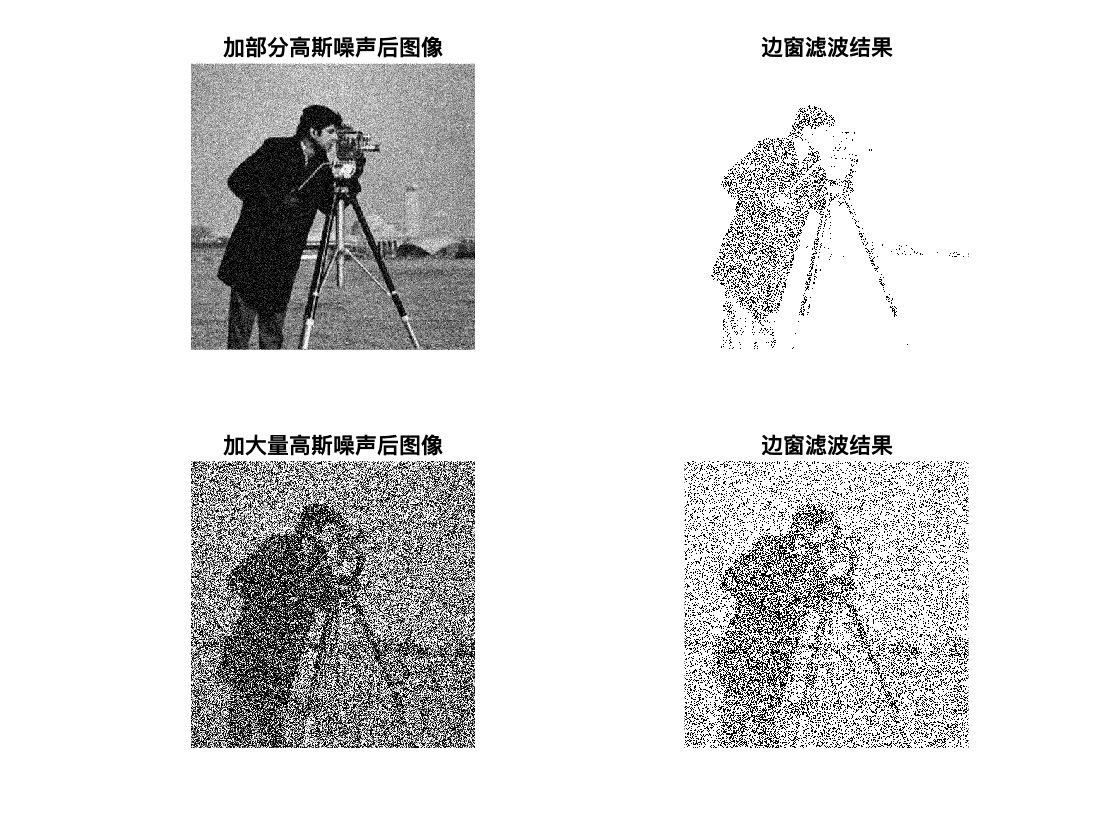
\includegraphics[width=9cm]{SWBF滤波结果.png} 	
	}
	\caption{边窗滤波仿真结果}
	\label{pic7}
\end{figure}

图\ref{pic7}左边一列显示了对灰度图像添加不同水平的高斯噪声后的结果,可以明显看出,随着加入的高斯噪声的增多,图片的模糊程度逐渐增加,图片愈发难以辨认。

图\ref{pic7}右边一列显示了添加高斯噪声后的灰度图片进行边窗滤波的结果。通过对比可以看出,经过边窗滤波后的图像较好地保留了原始图像的轮廓。

\begin{figure}[htbp]
	\centerline{
		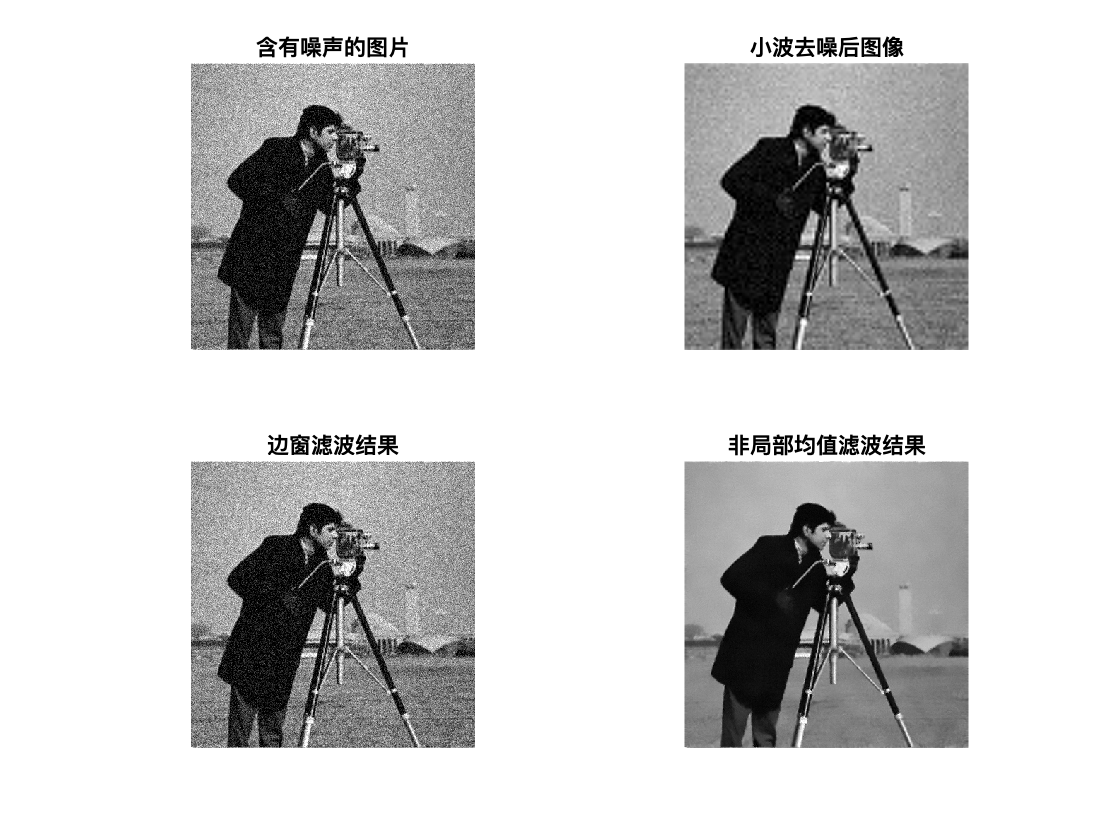
\includegraphics[width=9cm]{compare.png} 	
	}
	\caption{边窗滤波同部分滤波器对比结果}
	\label{pic8}
\end{figure}
图\ref{pic8}显示了边窗滤波同小波去噪,非局部均值滤波的比较。边窗滤波迭代次数为1次。可以看出,经过边窗滤波后的图像轮廓边缘更加突出,人物的手同其余两个滤波器相比更加突出。

\begin{figure}[htbp]
	\centerline{
		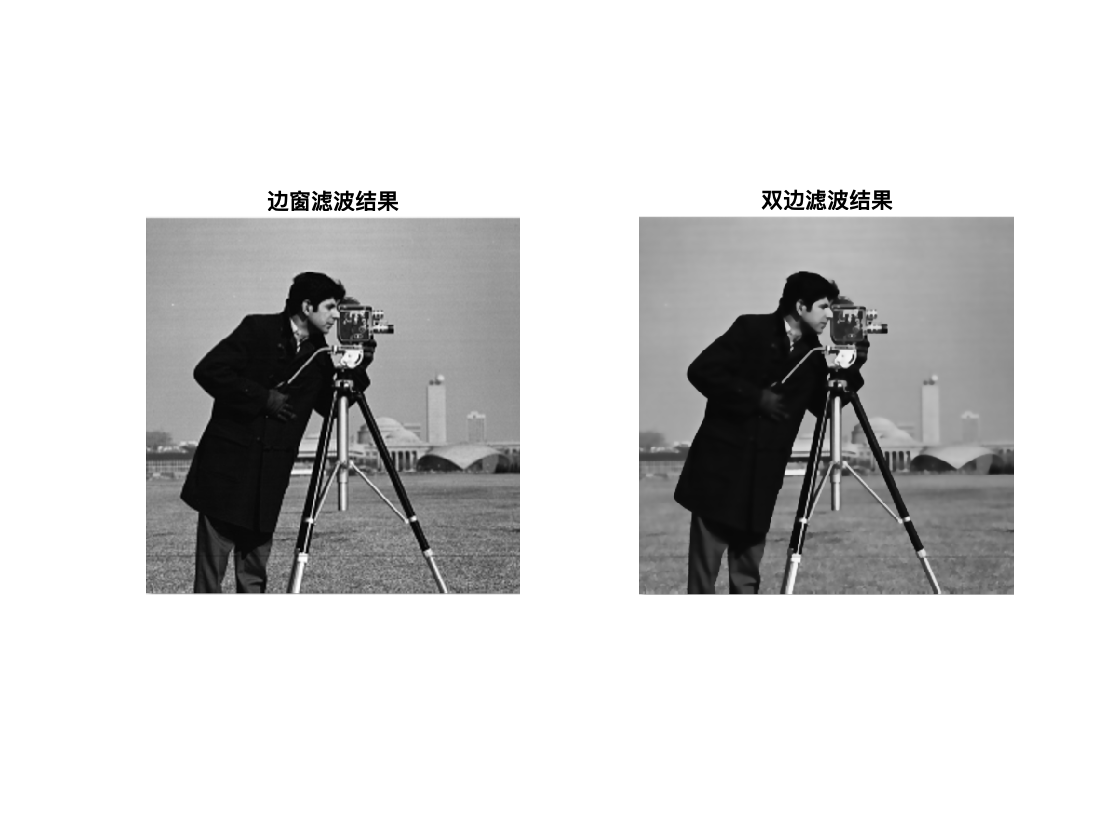
\includegraphics[width=9cm]{SWBF_BF.png} 	
	}
	\caption{边窗滤波同双边滤波对比结果}
	\label{pic9}
\end{figure}

\begin{figure}[htbp]
	\centerline{
		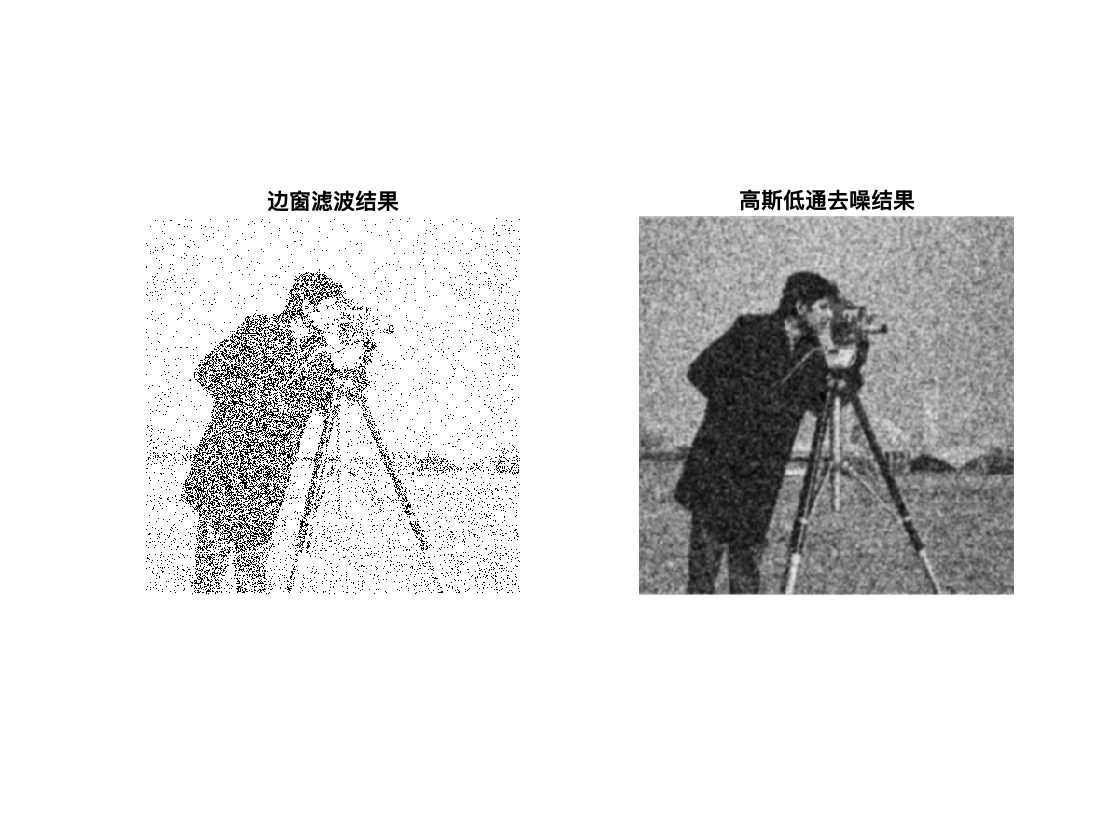
\includegraphics[width=9cm]{SWBF_GL.png} 	
	}
	\caption{边窗滤波同高斯低通滤波对比结果}
	\label{pic10}
\end{figure}

图\ref{pic9}与图\ref{pic10}显示了边窗滤波分别同双边滤波,高斯低通滤波的比较。边窗滤波迭代次数为1次。同双边滤波后的图像相比,经过边窗滤波后的图像轮廓边缘更加突出,没有出现边缘轮廓虚化的现象,同时人物的手同双边滤波后的图像相比更加突出。相同噪声条件下,高斯低通滤波后的图像出现了边缘轮廓虚化的现象,相反,经过边窗滤波后的图像很好的保留了图像的轮廓,没有出现虚化的现象,然而,相同噪声条件下边窗滤波滤波效果没有高斯低通滤波好。

\section{维纳滤波仿真结果}
\begin{figure}[htbp]
	\centerline{
		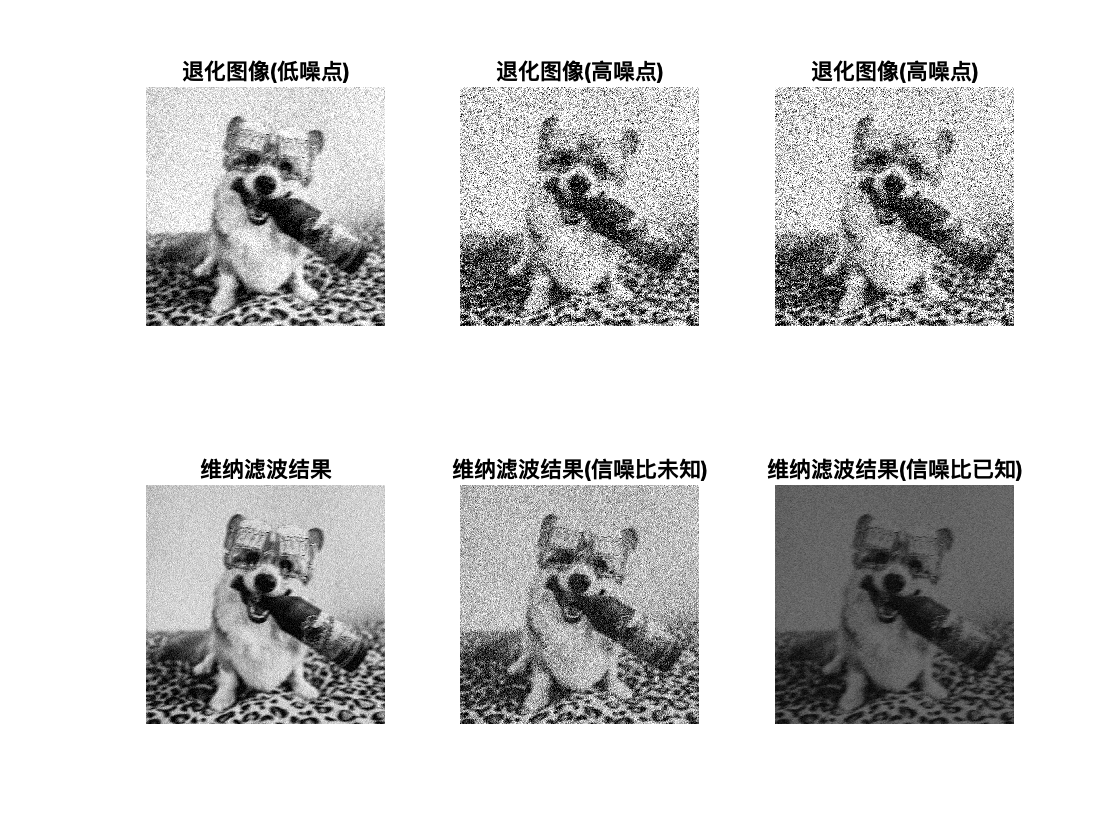
\includegraphics[width=9cm]{WF.png} 	
	}
	\caption{维纳滤波仿真结果}
	\label{pic11}
\end{figure}

图\ref{pic11}展示了对模糊的退化图像进行维纳滤波\cite{b7}\cite{b8}的仿真结果。其中,图片第一行显示了对图像添加高斯低通滤波,再加上高斯噪声后的三幅退化图像。可以看出,添加对应噪声后,图像出现了模糊的现象。第一行右边两张图片进行的加噪处理相同,目的为了进行维纳滤波的对比。第二行的三张图片显示了分别对第一行三张图片添加不同程度的维纳滤波后的结果。其中第二行第一张图片为第一行第一张图片进行维纳滤波处理的结果,以此类推。

通过对比第一列图片可以看出,在低噪点同时已知信噪比的条件下,经过维纳滤波后的图像复原效果较好,维纳滤波对模糊的抑制程度较高,但图像仍然存在部分模糊的现象。

第二列与第三列为对原始图像添加大量噪点后进行维纳滤波的结果。其中第二列的假设滤波过程的信噪比未知,第三列为已知信噪比条件下的滤波结果。通过对比可以看出,信噪比未知条件下的维纳滤波效果相比较信噪比已知条件下的维纳滤波效果较差,但在高噪声的条件下,已知信噪比的维纳滤波结果出现了背景黑化的现象。

\section{总结}
本实践报告为数字图像处理课程中期实践报告,内容涵盖图像增强、图像去噪、边窗滤波与维纳滤波等。通过实际实践编程仿真加深了对图像处理的认识,同时学习并掌握了图像处理的基础知识。


\begin{thebibliography}{00}
	\bibitem{b1} Acharya, Tinku, and Ajoy K. Ray. Image processing: principles and applications. John Wiley \& Sons, 2005.
	\bibitem{b2} Pizer, Stephen M., et al. "Adaptive histogram equalization and its variations." Computer vision, graphics, and image processing 39.3 (1987): 355-368.
	\bibitem{b3} Portilla, Javier, et al. "Image denoising using scale mixtures of Gaussians in the wavelet domain." IEEE Transactions on Image processing 12.11 (2003): 1338-1351.
	\bibitem{b4} Tomasi, Carlo, and Roberto Manduchi. "Bilateral filtering for gray and color images." Sixth international conference on computer vision (IEEE Cat. No. 98CH36271). IEEE, 1998.
	\bibitem{b5} Buades, Antoni, Bartomeu Coll, and J-M. Morel. "A non-local algorithm for image denoising." 2005 IEEE Computer Society Conference on Computer Vision and Pattern Recognition (CVPR'05). Vol. 2. IEEE, 2005.
	\bibitem{b6} Yin, Hui, Yuanhao Gong, and Guoping Qiu. "Side window filtering." Proceedings of the IEEE/CVF Conference on Computer Vision and Pattern Recognition. 2019.
	\bibitem{b7} Wiener, Norbert, et al. Extrapolation, interpolation, and smoothing of stationary time series: with engineering applications. Vol. 113. No. 21. Cambridge, MA: MIT press, 1949.
	\bibitem{b8} Kumar, Suresh, et al. "Performance comparison of median and wiener filter in image de-noising." International Journal of Computer Applications 12.4 (2010): 27-31.
\end{thebibliography}
\end{document}
